\documentclass[11pt,a4paper]{article}

\usepackage[a4paper,top=20mm,bottom=21mm,left=19mm,right=19mm]{geometry}
\usepackage{graphicx}
\usepackage[table]{xcolor}
\usepackage{booktabs}
\usepackage{tabularx}
\usepackage{array}
\usepackage{amsmath}
\usepackage{caption}
\usepackage{titlesec}
\usepackage[most]{tcolorbox}
\usepackage{enumitem}
\usepackage{hyperref}
\usepackage{xepersian}

\settextfont[
  Path={C:/Users/ROG/AppData/Local/Microsoft/Windows/Fonts/},
  UprightFont={XB Niloofar.ttf},
  BoldFont={XB NiloofarBd.ttf},
  ItalicFont={XB NiloofarIt.ttf},
  BoldItalicFont={XB NiloofarBdIt.ttf}
]{XB Niloofar}
\setlatintextfont{TeX Gyre Heros}
\setdigitfont[
  Path={C:/Users/ROG/AppData/Local/Microsoft/Windows/Fonts/},
  UprightFont={XB Niloofar.ttf},
  BoldFont={XB NiloofarBd.ttf}
]{XB Niloofar}

\definecolor{ink}{HTML}{162335}
\definecolor{deepblue}{HTML}{176B87}
\definecolor{mint}{HTML}{64CCC5}
\definecolor{coral}{HTML}{EF6262}
\definecolor{paperblue}{HTML}{EEF8FB}
\definecolor{papermint}{HTML}{F2FBFA}
\definecolor{softgray}{HTML}{F3F5F7}
\definecolor{goodgreen}{HTML}{2E8B72}


\hypersetup{
  colorlinks=true,
  linkcolor=deepblue,
  urlcolor=coral,
  pdftitle={گزارش فارسی پروژه پردازش صوت و تصویر چاه},
  pdfsubject={درس سیگنال‌ها و سیستم‌ها},
  pdfauthor={شایان صالحی, ۴۰۴۲۰۳۵۰۹}
}

\graphicspath{{../figures/}{../outputs/images/}}
\captionsetup{font=small,labelfont=bf,justification=centering}
\setlength{\parindent}{0pt}
\setlength{\parskip}{5pt}
\setlength{\tabcolsep}{5pt}
\renewcommand{\arraystretch}{1.25}

\titleformat{\section}
  {\Large\bfseries\color{deepblue}}
  {\thesection}{0.55em}{}
  [\vspace{2pt}\color{mint}\titlerule]
\titleformat{\subsection}
  {\large\bfseries\color{deepblue}}
  {\thesubsection}{0.5em}{}

\newtcolorbox{ideaBox}[1][]{
  enhanced,
  colback=papermint,
  colframe=mint,
  boxrule=0.8pt,
  arc=2mm,
  left=3mm,right=3mm,top=2mm,bottom=2mm,
  title=#1,
  coltitle=ink,
  fonttitle=\bfseries
}

\newtcolorbox{resultBox}[1][]{
  enhanced,
  colback=paperblue,
  colframe=deepblue,
  boxrule=0.8pt,
  arc=2mm,
  left=3mm,right=3mm,top=2mm,bottom=2mm,
  title=#1,
  coltitle=ink,
  fonttitle=\bfseries
}

\newcommand{\en}[1]{\lr{#1}}
\newcommand{\metric}[1]{\textcolor{goodgreen}{\bfseries #1}}

\begin{document}
\pagestyle{plain}

\begin{titlepage}
\thispagestyle{empty}
\vspace*{12mm}

{\color{deepblue}\rule{\textwidth}{2.2pt}}
\vspace{9mm}

{\Huge\bfseries\color{ink}
گزارش پروژه‌ی عملی اول
\par}
\vspace{5mm}
{\LARGE\color{deepblue}
بهبود صوت مکالمه و تشخیص شکستگی در تصویر چاه
\par}

\vspace{7mm}
{\large درس سیگنال‌ها و سیستم‌ها}

\vspace{8mm}

\begin{center}
\begin{tcolorbox}[
  width=0.78\textwidth,
  colback=papermint,
  colframe=mint,
  boxrule=0.9pt,
  arc=2.5mm,
  left=4mm,right=4mm,top=2.5mm,bottom=2.5mm
]
\centering\large
نام دانشجو: \textbf{شایان صالحی}
\qquad
شماره دانشجویی: \textbf{۴۰۴۲۰۳۵۰۹}
\end{tcolorbox}
\end{center}

\vspace{8mm}

\begin{tcolorbox}[
  colback=paperblue,
  colframe=deepblue,
  boxrule=1pt,
  arc=3mm,
  left=6mm,right=6mm,top=5mm,bottom=5mm
]
\large
در این پروژه دو مسئله‌ی واقعی را با ابزارهای کلاسیک پردازش سیگنال حل کردیم. اول سه فایل مکالمه را از نظر سکوت، نویز، محدودیت پهنای باند و اکو بررسی و تمیز کردیم. بعد سراغ تصاویر بازشده‌ی دیواره‌ی چاه رفتیم و با تقویت کنتراست، آشکارسازی رگه، عملیات مورفولوژیک و آزمون پیوستگی، شکستگی‌های اصلی را جدا کردیم.
\end{tcolorbox}

\vfill

\begin{center}
\begin{tabularx}{0.92\textwidth}{>{\centering\arraybackslash}X >{\centering\arraybackslash}X >{\centering\arraybackslash}X}
\cellcolor{deepblue}\color{white}\bfseries ۳ فایل صوتی &
\cellcolor{deepblue}\color{white}\bfseries ۲ تصویر اصلی &
\cellcolor{deepblue}\color{white}\bfseries ۸ تصویر آزمایشی\\
\cellcolor{paperblue}پردازش کامل و خروجی \en{WAV} &
\cellcolor{paperblue}ماسک و تصویر هم‌پوشانی &
\cellcolor{paperblue}بررسی تعمیم‌پذیری
\end{tabularx}
\end{center}

\vfill

{\small\color{ink}
این گزارش توضیح ساده و ارائه‌محورِ همان نوت‌بوک اجراشده است. همه‌ی عددها و شکل‌ها مستقیماً از اجرای نهایی نوت‌بوک آمده‌اند.
}

\vspace{7mm}
{\color{coral}\rule{\textwidth}{1.3pt}}
\end{titlepage}

\section{ایده‌ی کلی پروژه}

هدف این نبود که یک فیلتر خیلی سنگین روی داده بگذاریم و فقط خروجی نهایی را نشان بدهیم. تلاش کردیم هر تصمیم قابل دیدن باشد. در بخش صوت، سکوت، فرکانس‌های خارج از باند، نویز ایستا، اکو و تغییر بلندی صدا جداگانه بررسی شدند. در بخش تصویر هم ابتدا پیکسل‌های شبیه رگه پیدا شدند و بعد طول و پیوستگی آن‌ها تصمیم نهایی را ساخت.

\begin{ideaBox}[چرا این روش مناسب بود؟]
برای فایل‌های صوتی مرجعِ تمیز نداریم و برای تصاویر هم ماسک دستی وجود ندارد. پس بهتر است روش توضیح‌پذیر باشد و بتوانیم با نمودار، معیار و خروجی میانی نشان بدهیم چرا چیزی حذف یا نگه داشته شده است.
\end{ideaBox}

\begin{figure}[ht]
\centering
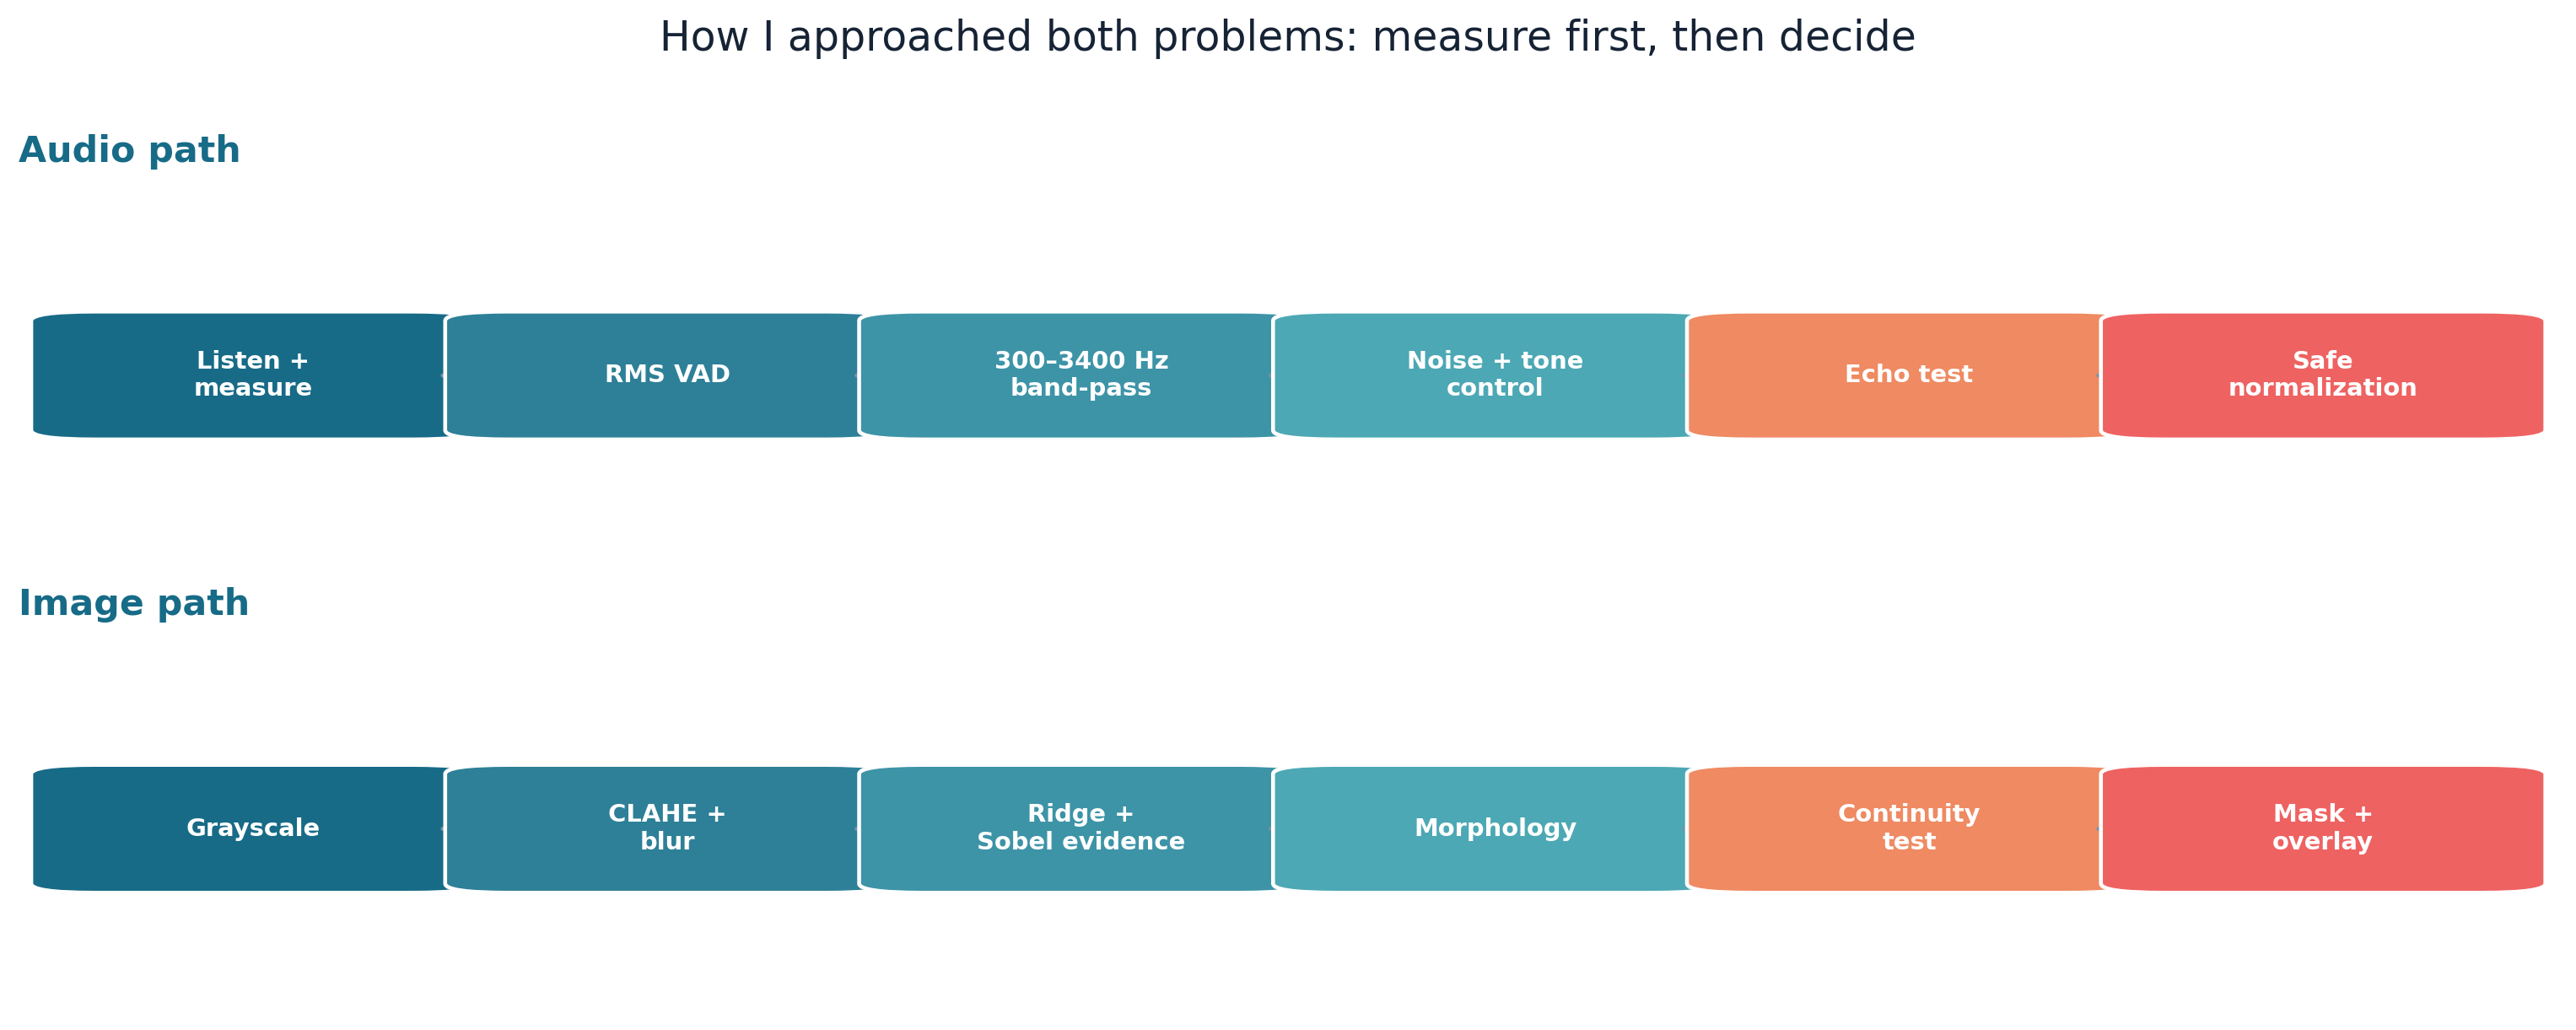
\includegraphics[width=\textwidth]{00_workflow_map.png}
\caption{نقشه‌ی دو مسیر پردازش. نوشته‌های داخل شکل انگلیسی‌اند چون همین شکل در نوت‌بوک اصلی استفاده شده است.}
\end{figure}

در مسیر صوت، داده با نرخ نمونه‌برداری یکسان \en{22.05 kHz} خوانده شد. در مسیر تصویر هم اندازه‌ی کرنل‌ها به صورت نسبی انتخاب شد تا همان کد هم روی تصاویر پهن اصلی و هم روی نمونه‌های کوچک‌تر اجرا شود.

\clearpage
\section{بخش اول: شناخت فایل‌های صوتی}

\subsection{قبل از فیلتر چه دیدیم؟}

شکل زیر مهم‌ترین بخش تحلیل اولیه است. ستون سمت چپ موج زمانی را نشان می‌دهد و ناحیه‌های خیلی کم‌رنگ سبز همان قسمت‌هایی هستند که آشکارساز فعالیت صوتی به عنوان بخش فعال تشخیص داده است. ستون سمت راست طیف‌نگاره‌ی \en{STFT} است.

\begin{figure}[ht]
\centering
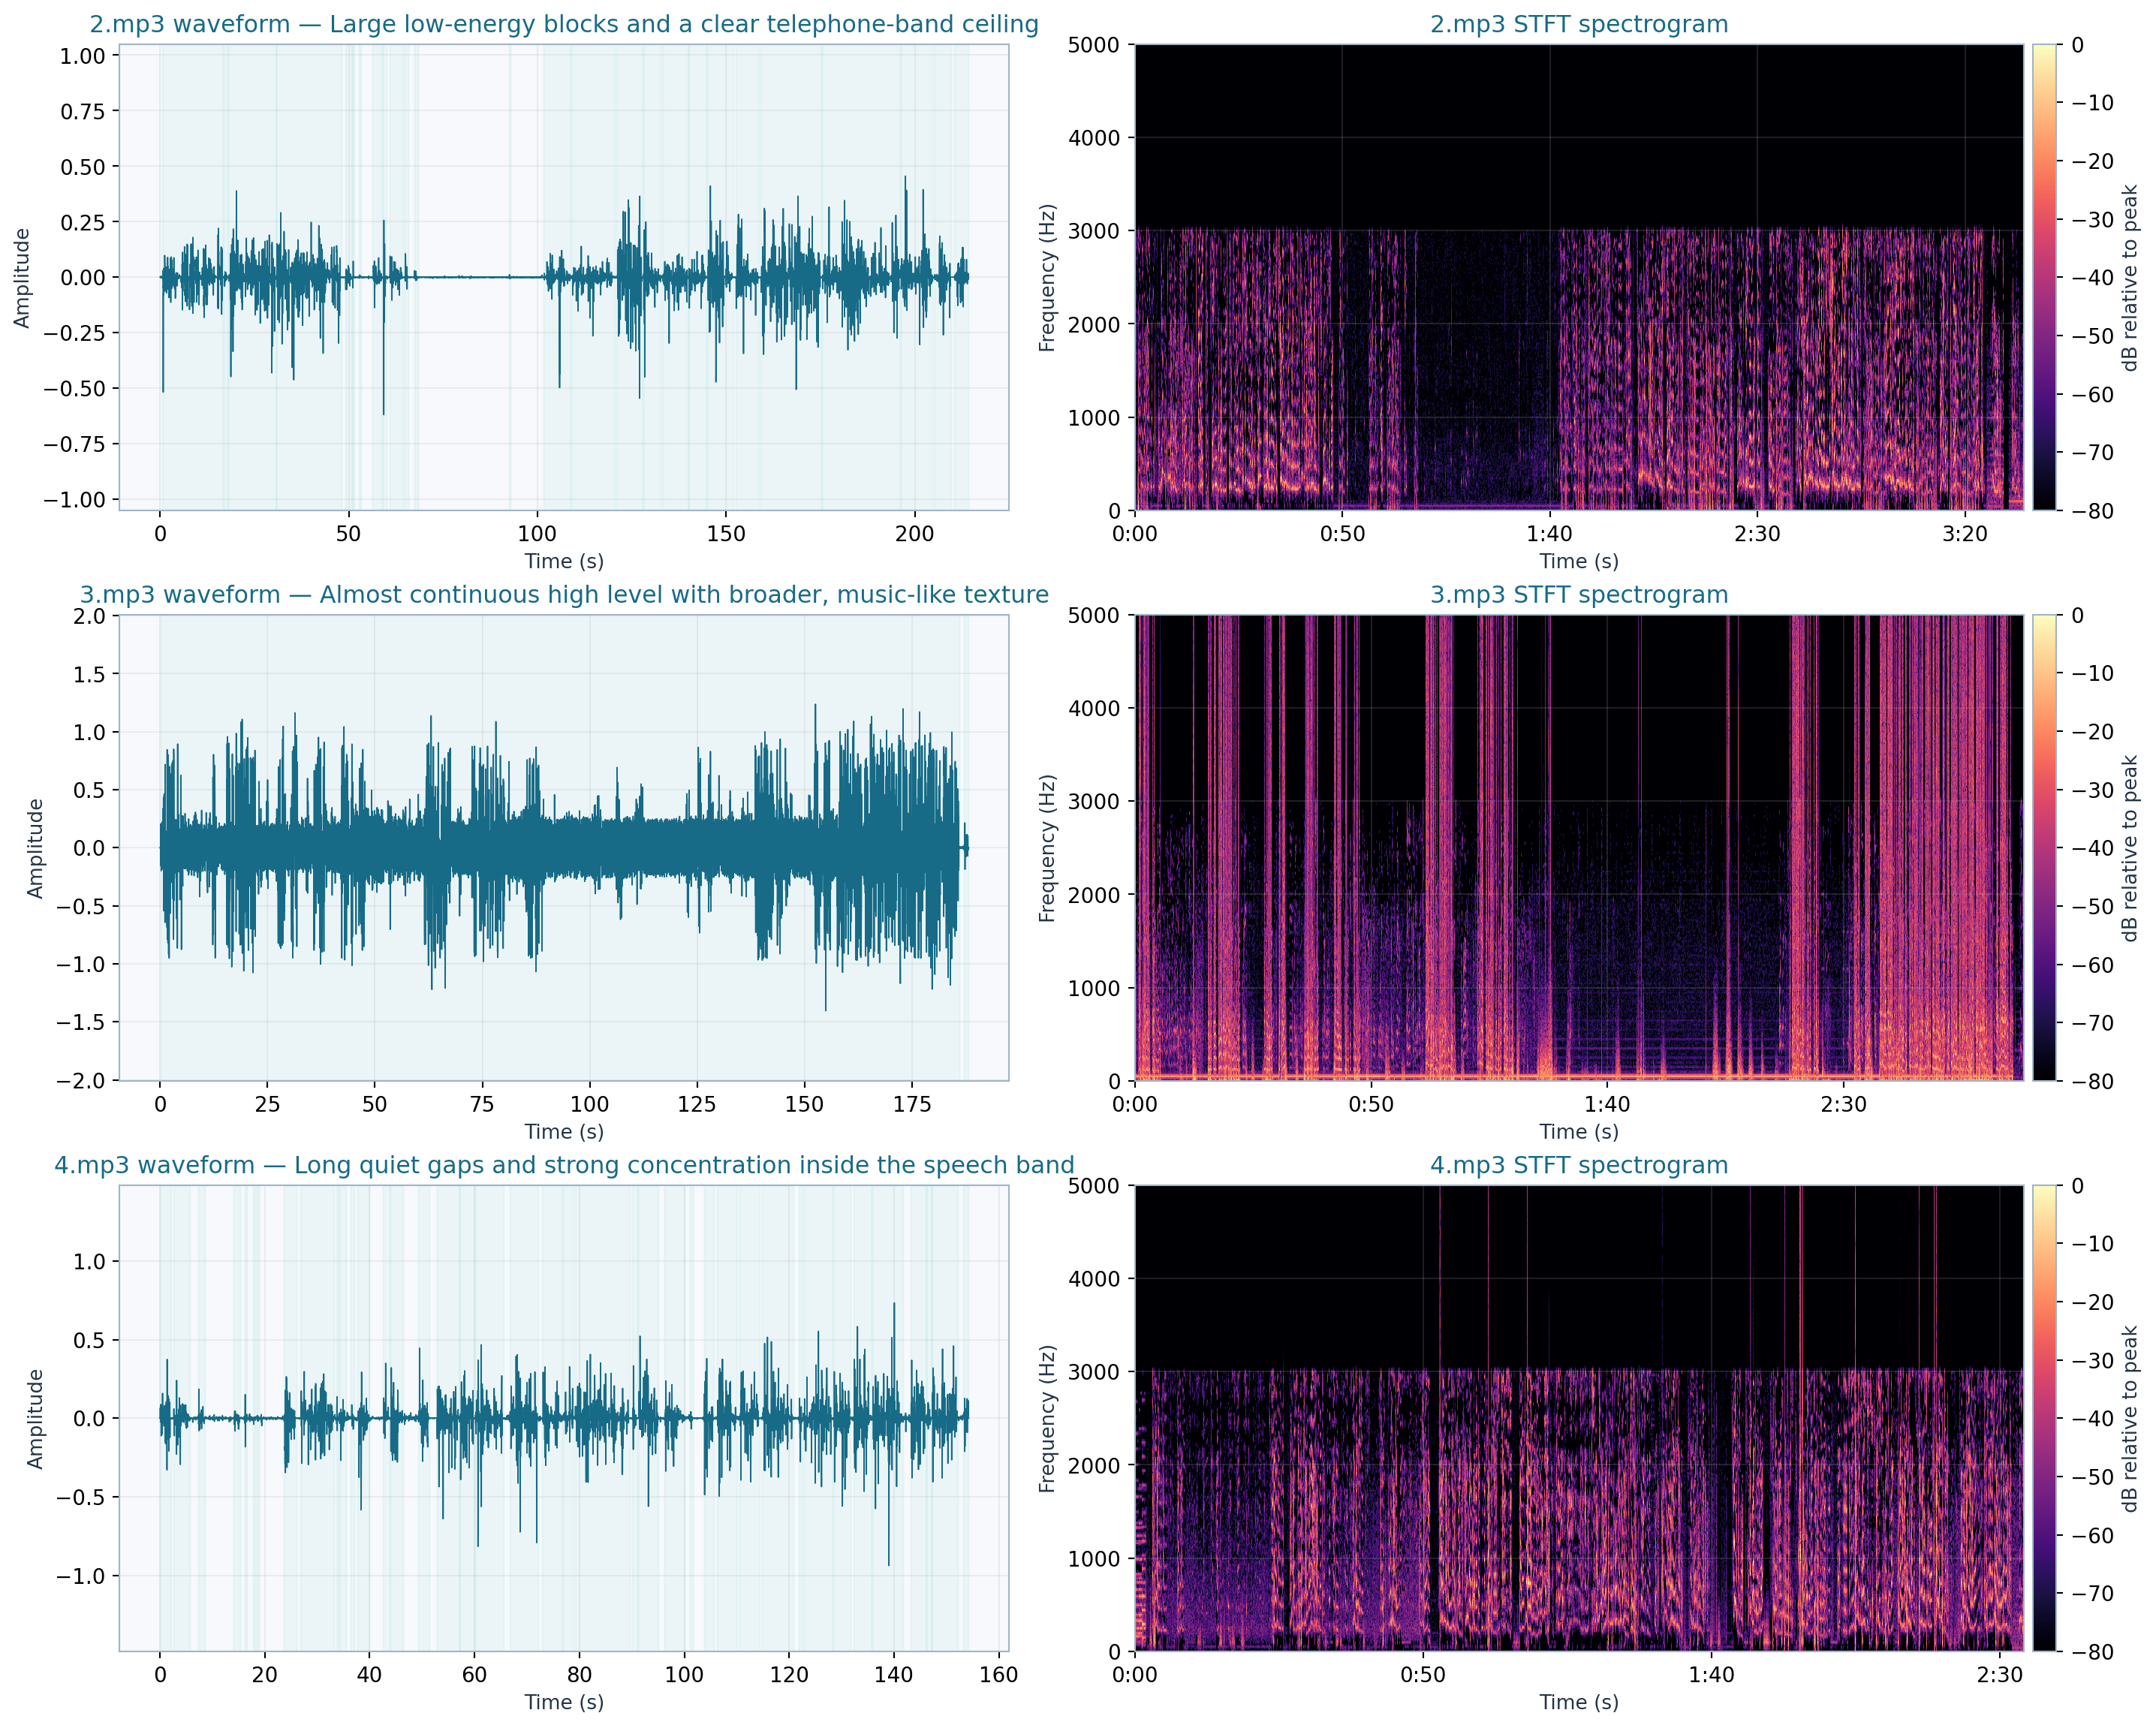
\includegraphics[width=0.96\textwidth]{01_audio_eda.png}
\caption{نمای زمانی و فرکانسی سه فایل صوتی قبل از پردازش}
\end{figure}

از این شکل سه نتیجه‌ی ساده می‌گیریم:

\begin{itemize}[rightmargin=6mm,itemsep=3pt]
  \item فایل‌های \en{2.mp3} و \en{4.mp3} چند بازه‌ی سکوت بلند دارند و انرژی اصلی آن‌ها تقریباً زیر \en{3 kHz} مانده است.
  \item فایل \en{3.mp3} تقریباً پیوسته و خیلی بلند است؛ بنابراین حذف سکوت در آن نقش کمی دارد.
  \item سقف باند تلفنی در فایل‌های ۲ و ۴ کاملاً دیده می‌شود. در فایل ۳ بافت فرکانسی پهن‌تر است و رفتار آن بیشتر به موسیقی انتظار یا صدای ترکیبی شبیه است.
\end{itemize}

\clearpage
\section{زنجیره‌ی بهبود صوت}

\subsection{آشکارسازی گفتار و حذف سکوت بلند}

برای هر فریم، مقدار \en{RMS} محاسبه شد:
\[
x_{\mathrm{RMS}}=
\sqrt{\frac{1}{N}\sum_{n=0}^{N-1}x^2[n]}.
\]

آستانه‌ی روشن‌شدن و خاموش‌شدن کمی با هم فرق دارد. این هیسترزیس کوچک باعث می‌شود تصمیم نزدیک مرز مدام صفر و یک نشود. فاصله‌های خیلی کوتاه پر شدند، قطعه‌های خیلی کوتاه حذف شدند و کمی حاشیه در ابتدا و انتهای گفتار نگه داشتیم تا کلمه‌ها بریده نشوند.

\subsection{فیلتر باندگذر}

یک فیلتر باتروورث مرتبه‌ی چهارم با باند \en{300--3400 Hz} استفاده شد. پیاده‌سازی به شکل \en{SOS} و با \en{sosfiltfilt} انجام شد تا هم پایداری عددی خوب باشد و هم فاز گفتار جابه‌جا نشود. این مرحله برای فایل‌های تلفنی خیلی قابل اعتماد است، چون محدوده‌ی مفید کانال را از قبل می‌شناسیم.

\subsection{کاهش نویز با تفریق طیفی}

از فریم‌های کم‌انرژی یک تخمین برای اندازه‌ی طیف نویز ساختیم و آن را از هر فریم کم کردیم:
\[
|\widehat{S}(m,k)|=
\max\left(|Y(m,k)|-\alpha\widehat{N}(k),\,
\beta |Y(m,k)|\right).
\]
پارامتر \(\beta\) یک کف طیفی کوچک نگه می‌دارد تا حفره‌های شدید و صدای فلزی ایجاد نشود.

\subsection{آزمون اکو و کنترل بلندی}

برای اکو، خودهمبستگی نرمال‌شده در بازه‌ی \en{40--350 ms} بررسی شد. اگر تأخیر و بهره‌ی تخمینی قابل قبول بود، تقریب معکوس
\[
\widehat{s}[n]=y[n]-a\,y[n-D]
\]
اعمال شد. این در واقع یک تصمیم محافظه‌کارانه است؛ چون خود گفتار هم تناوب دارد و هر قله‌ی همبستگی لزوماً اکو نیست. در پایان، \en{RMS} هدف تنظیم شد و سقف پیک \en{-1 dBFS} اجازه‌ی کلیپ‌شدن نداد.

\clearpage
\section{نتیجه‌های عددی صوت}

\begin{table}[ht]
\centering
\caption{تغییر طول و سطح سیگنال}
\rowcolors{2}{softgray}{white}
\begin{tabular}{c c c c c c}
\toprule
فایل & طول اولیه & طول نهایی & زمان حذف‌شده & \en{RMS} اولیه & \en{RMS} نهایی\\
\midrule
\en{2.mp3} & \en{214.23 s} & \en{168.30 s} & \metric{\en{21.4\%}} & \en{-23.95} & \en{-23.57}\\
\en{3.mp3} & \en{188.16 s} & \en{187.05 s} & \en{0.6\%} & \en{-9.35} & \en{-21.32}\\
\en{4.mp3} & \en{154.25 s} & \en{117.17 s} & \metric{\en{24.0\%}} & \en{-20.92} & \en{-24.00}\\
\bottomrule
\end{tabular}
\end{table}

\begin{table}[ht]
\centering
\caption{مقایسه‌ی نسبت انرژی باند گفتار و تخمین \en{SNR}}
\rowcolors{2}{paperblue}{white}
\begin{tabular}{c c c c c}
\toprule
فایل & باند گفتار قبل & باند گفتار بعد & \en{SNR} قبل & \en{SNR} بعد\\
\midrule
\en{2.mp3} & \en{77.3\%} & \metric{\en{98.1\%}} & \en{31.40 dB} & \metric{\en{42.99 dB}}\\
\en{3.mp3} & \en{30.5\%} & \metric{\en{98.1\%}} & \en{29.67 dB} & \en{29.89 dB}\\
\en{4.mp3} & \en{92.3\%} & \metric{\en{99.6\%}} & \en{23.74 dB} & \metric{\en{29.05 dB}}\\
\bottomrule
\end{tabular}
\end{table}

\begin{resultBox}[برداشت ساده از جدول‌ها]
حذف سکوت برای فایل‌های ۲ و ۴ کاملاً اثرگذار بود، ولی در فایل ۳ تقریباً چیزی برای حذف وجود نداشت. فیلتر باندگذر در هر سه فایل سهم انرژی باند گفتار را به بیشتر از ۹۸ درصد رساند. تخمین \en{SNR} در فایل ۲ حدود \en{11.6 dB} و در فایل ۴ حدود \en{5.3 dB} بهتر شد. در فایل ۳ بهبود \en{SNR} کوچک است، چون بیشتر زمان فایل فعال و پرانرژی است.
\end{resultBox}

برای فایل ۳ یک تأخیر \en{64 ms} با بهره‌ی کوچک \en{0.016} پذیرفته شد و فیلتر معکوس ضعیف اعمال شد. نامزدهای فایل‌های ۲ و ۴ بهره‌ی خیلی کمی داشتند و عمداً اعمال نشدند. این رفتار بهتر از آن است که برای گرفتن یک عدد ظاهراً بهتر، گفتار را بی‌دلیل خراب کنیم.

\clearpage
\section{مقایسه‌ی قبل و بعد برای هر فایل}

\subsection{فایل \en{2.mp3}}

\begin{figure}[ht]
\centering
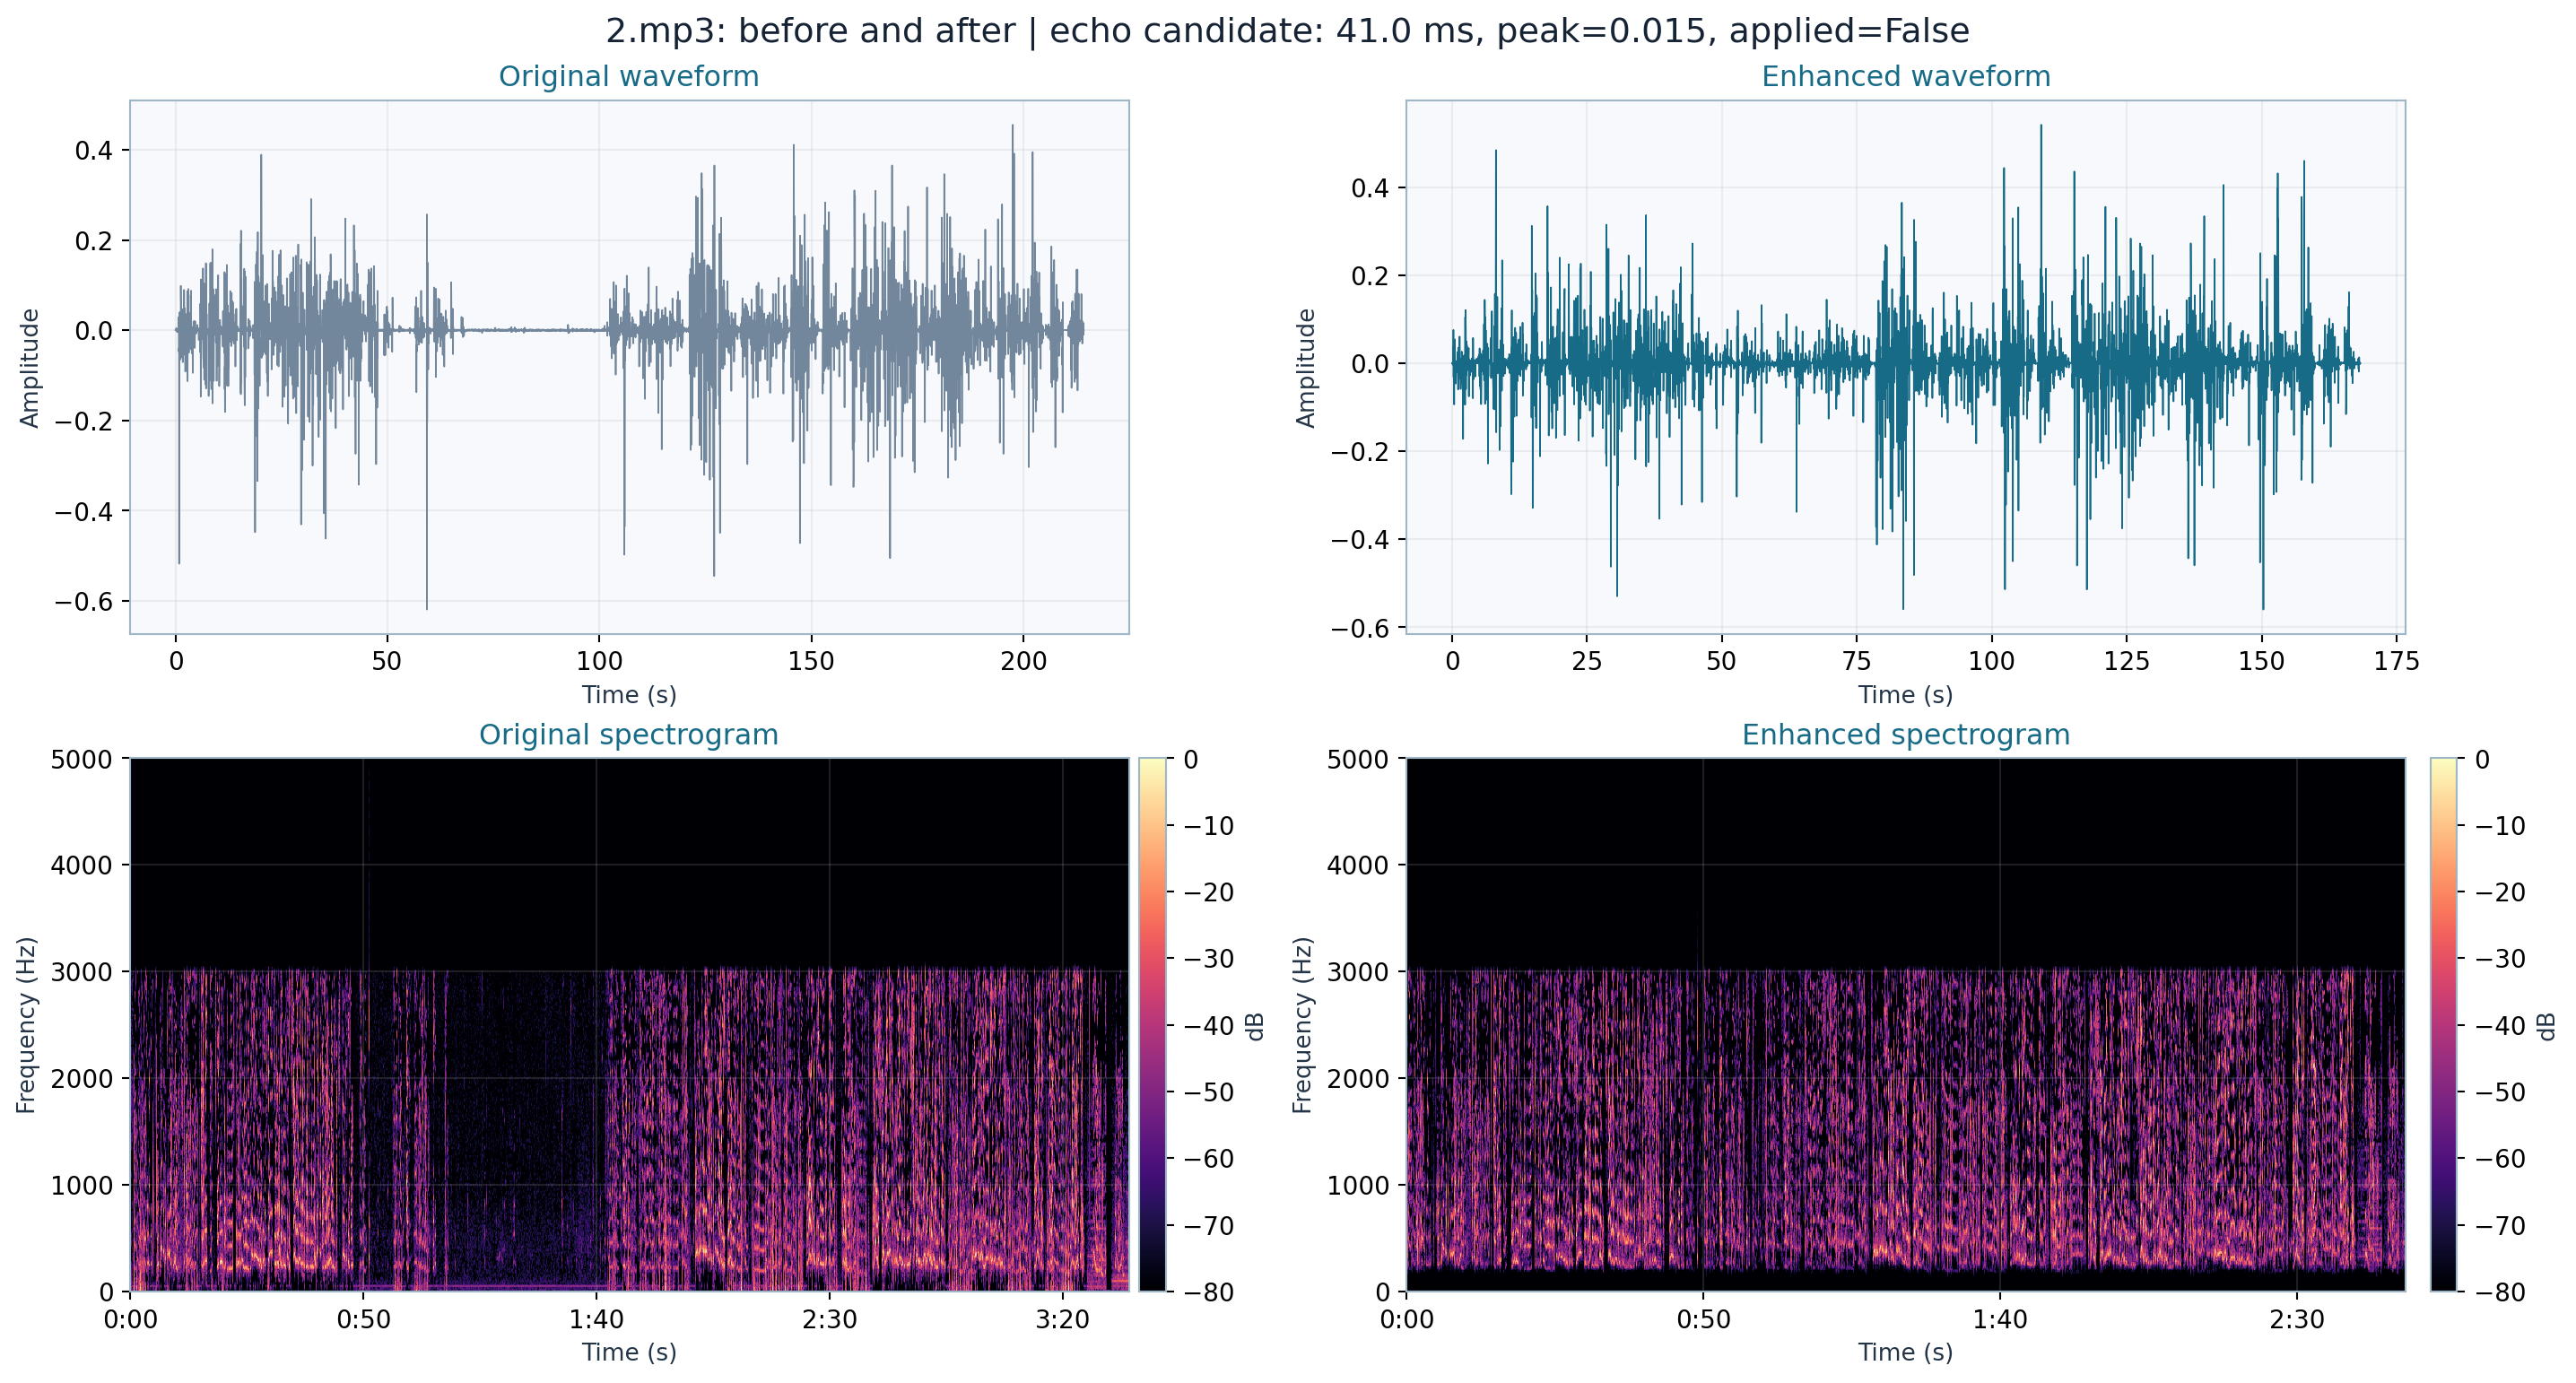
\includegraphics[width=0.96\textwidth]{audio_2_before_after.png}
\caption{مقایسه‌ی موج زمانی و طیف‌نگاره‌ی فایل ۲}
\end{figure}

بازه‌ی سکوت بزرگِ وسط فایل تقریباً حذف شده است. بعد از پردازش، انرژی بالاتر از باند تلفنی کم شده و کف نویز در ناحیه‌های بدون گفتار پایین‌تر است. بهترشدن \en{SNR} تخمینی در این فایل از همه واضح‌تر بود.

\clearpage
\subsection{فایل \en{3.mp3}}

\begin{figure}[ht]
\centering
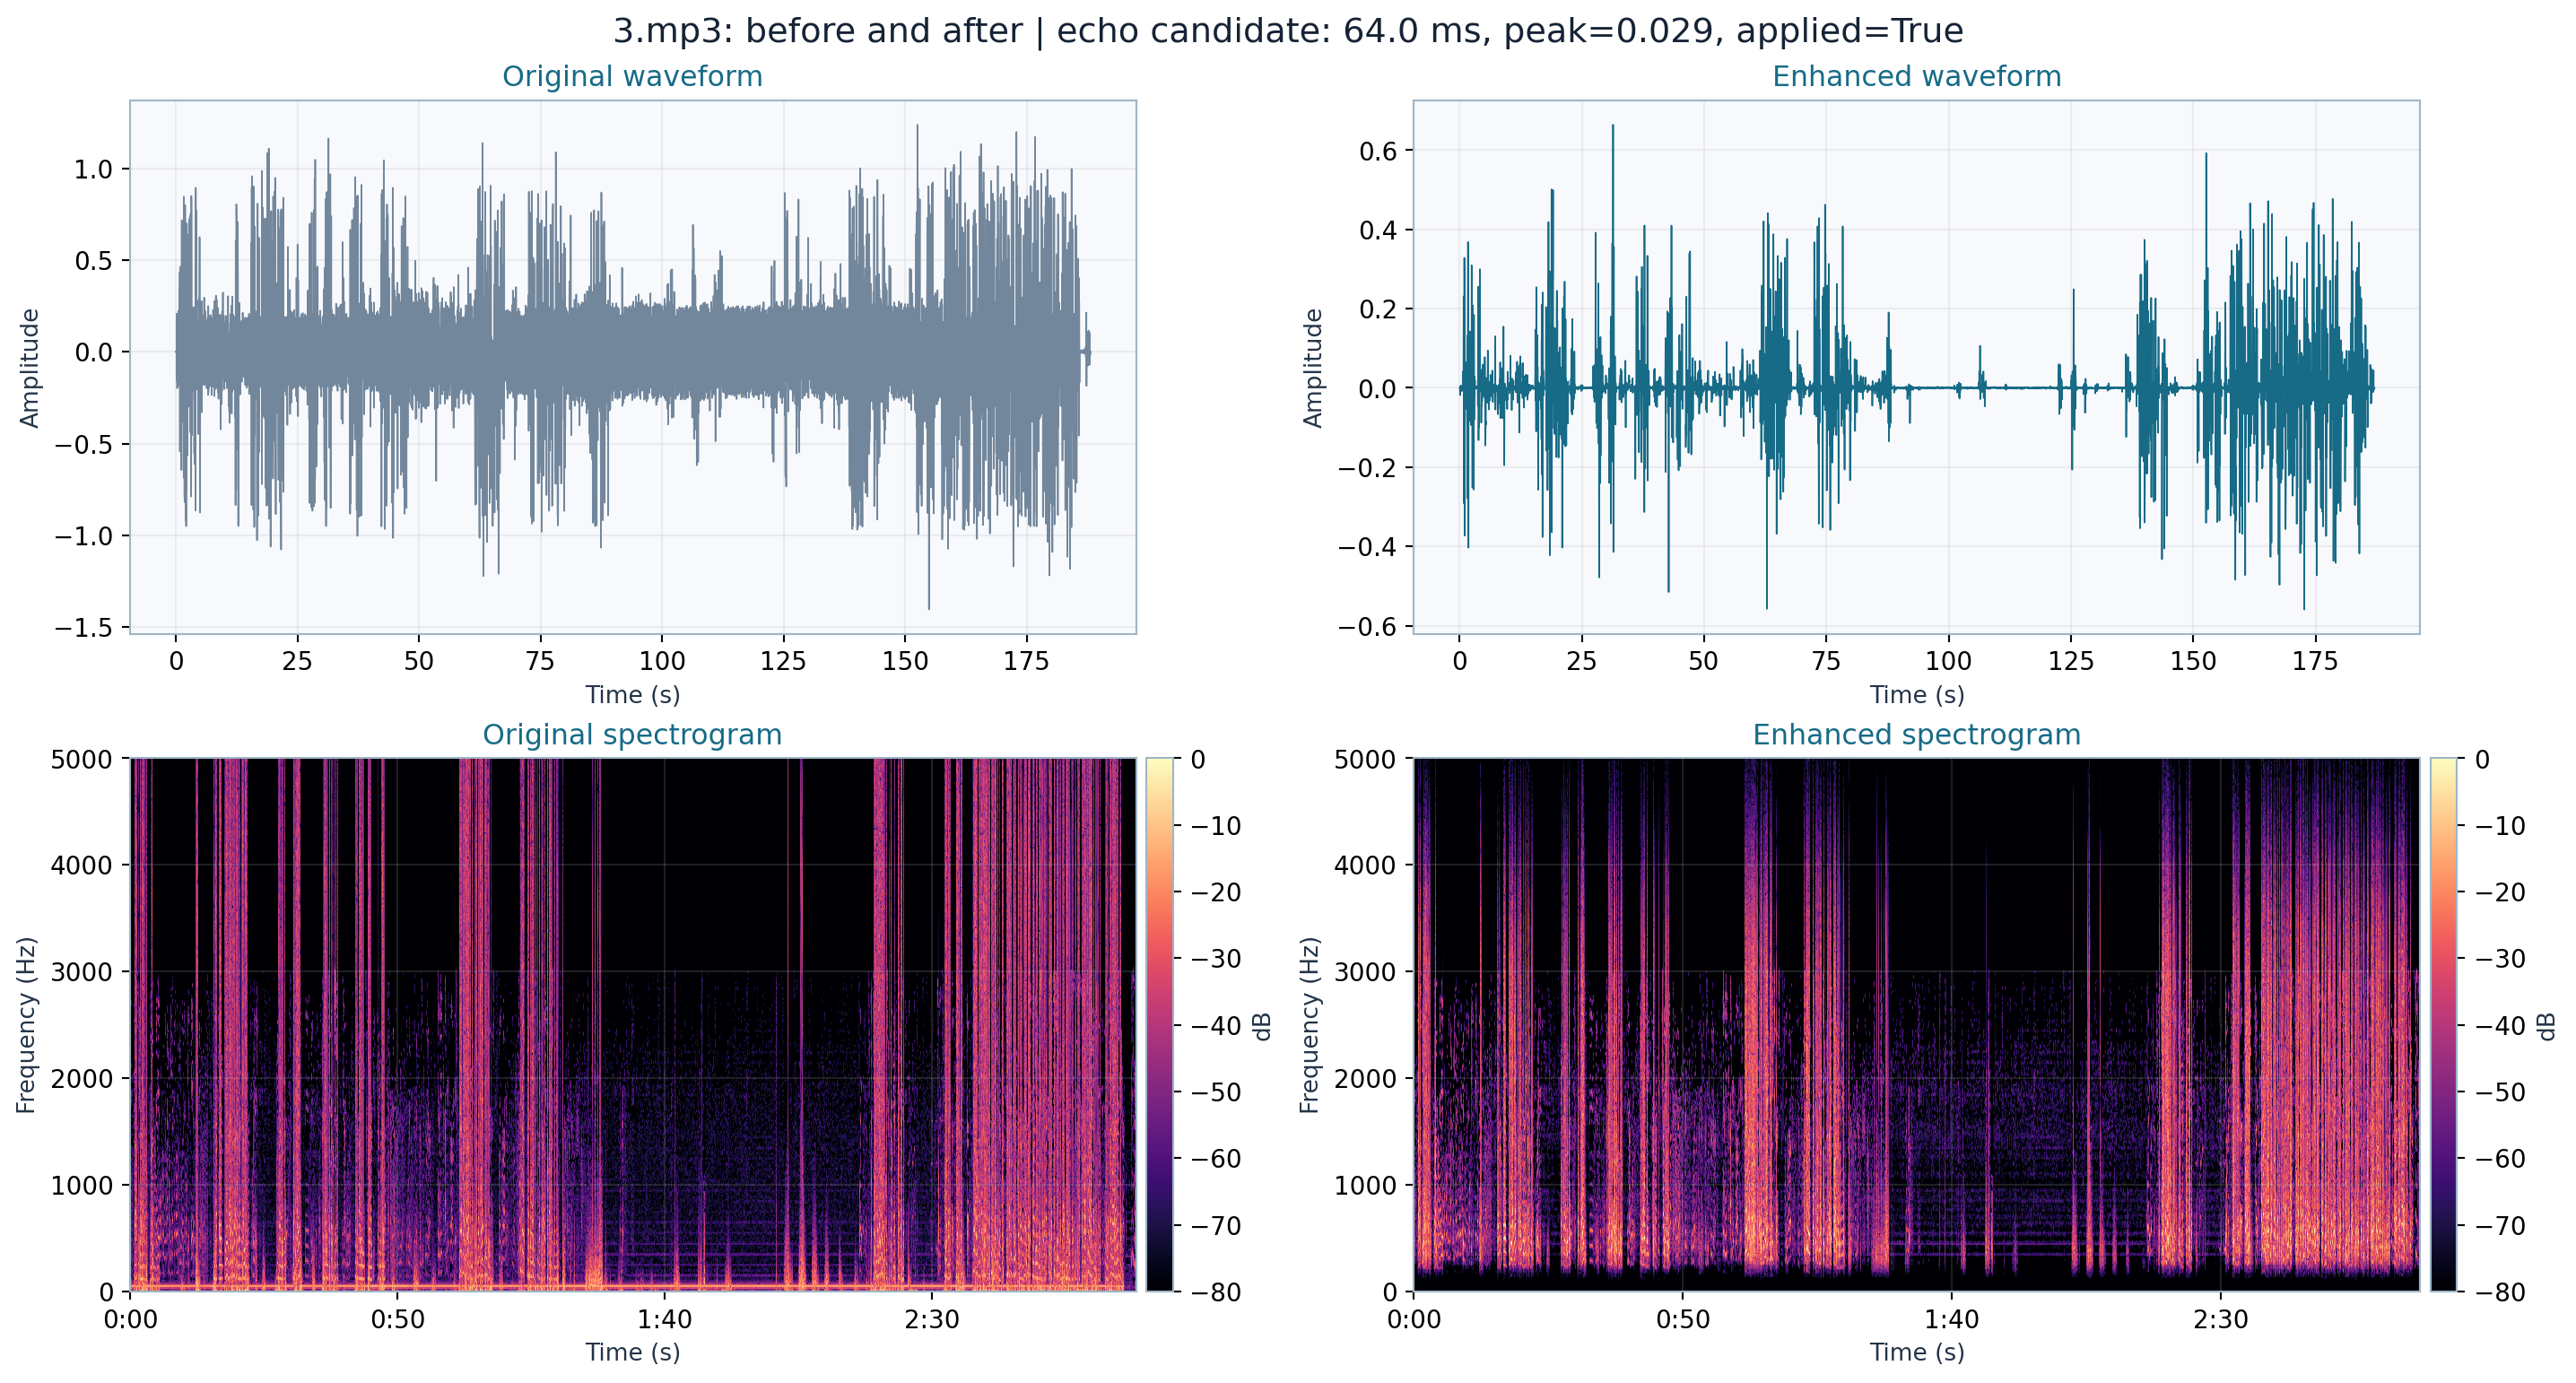
\includegraphics[width=0.96\textwidth]{audio_3_before_after.png}
\caption{مقایسه‌ی موج زمانی و طیف‌نگاره‌ی فایل ۳}
\end{figure}

طول این فایل تقریباً ثابت مانده، چون فعالیت صوتی پیوسته است. تغییر اصلی در محدودشدن باند، کم‌شدن مؤلفه‌های خارج از محدوده‌ی گفتار و یک اصلاح خیلی ضعیف برای اکو است. افت \en{RMS} نهایی نکته‌ی منفی نیست؛ فایل اولیه بیش از حد بلند بود و حتی پیک‌های بالاتر از یک داشت. نرمال‌سازی، خروجی را بدون کلیپ در محدوده‌ی امن قرار داد.

\clearpage
\subsection{فایل \en{4.mp3}}

\begin{figure}[ht]
\centering
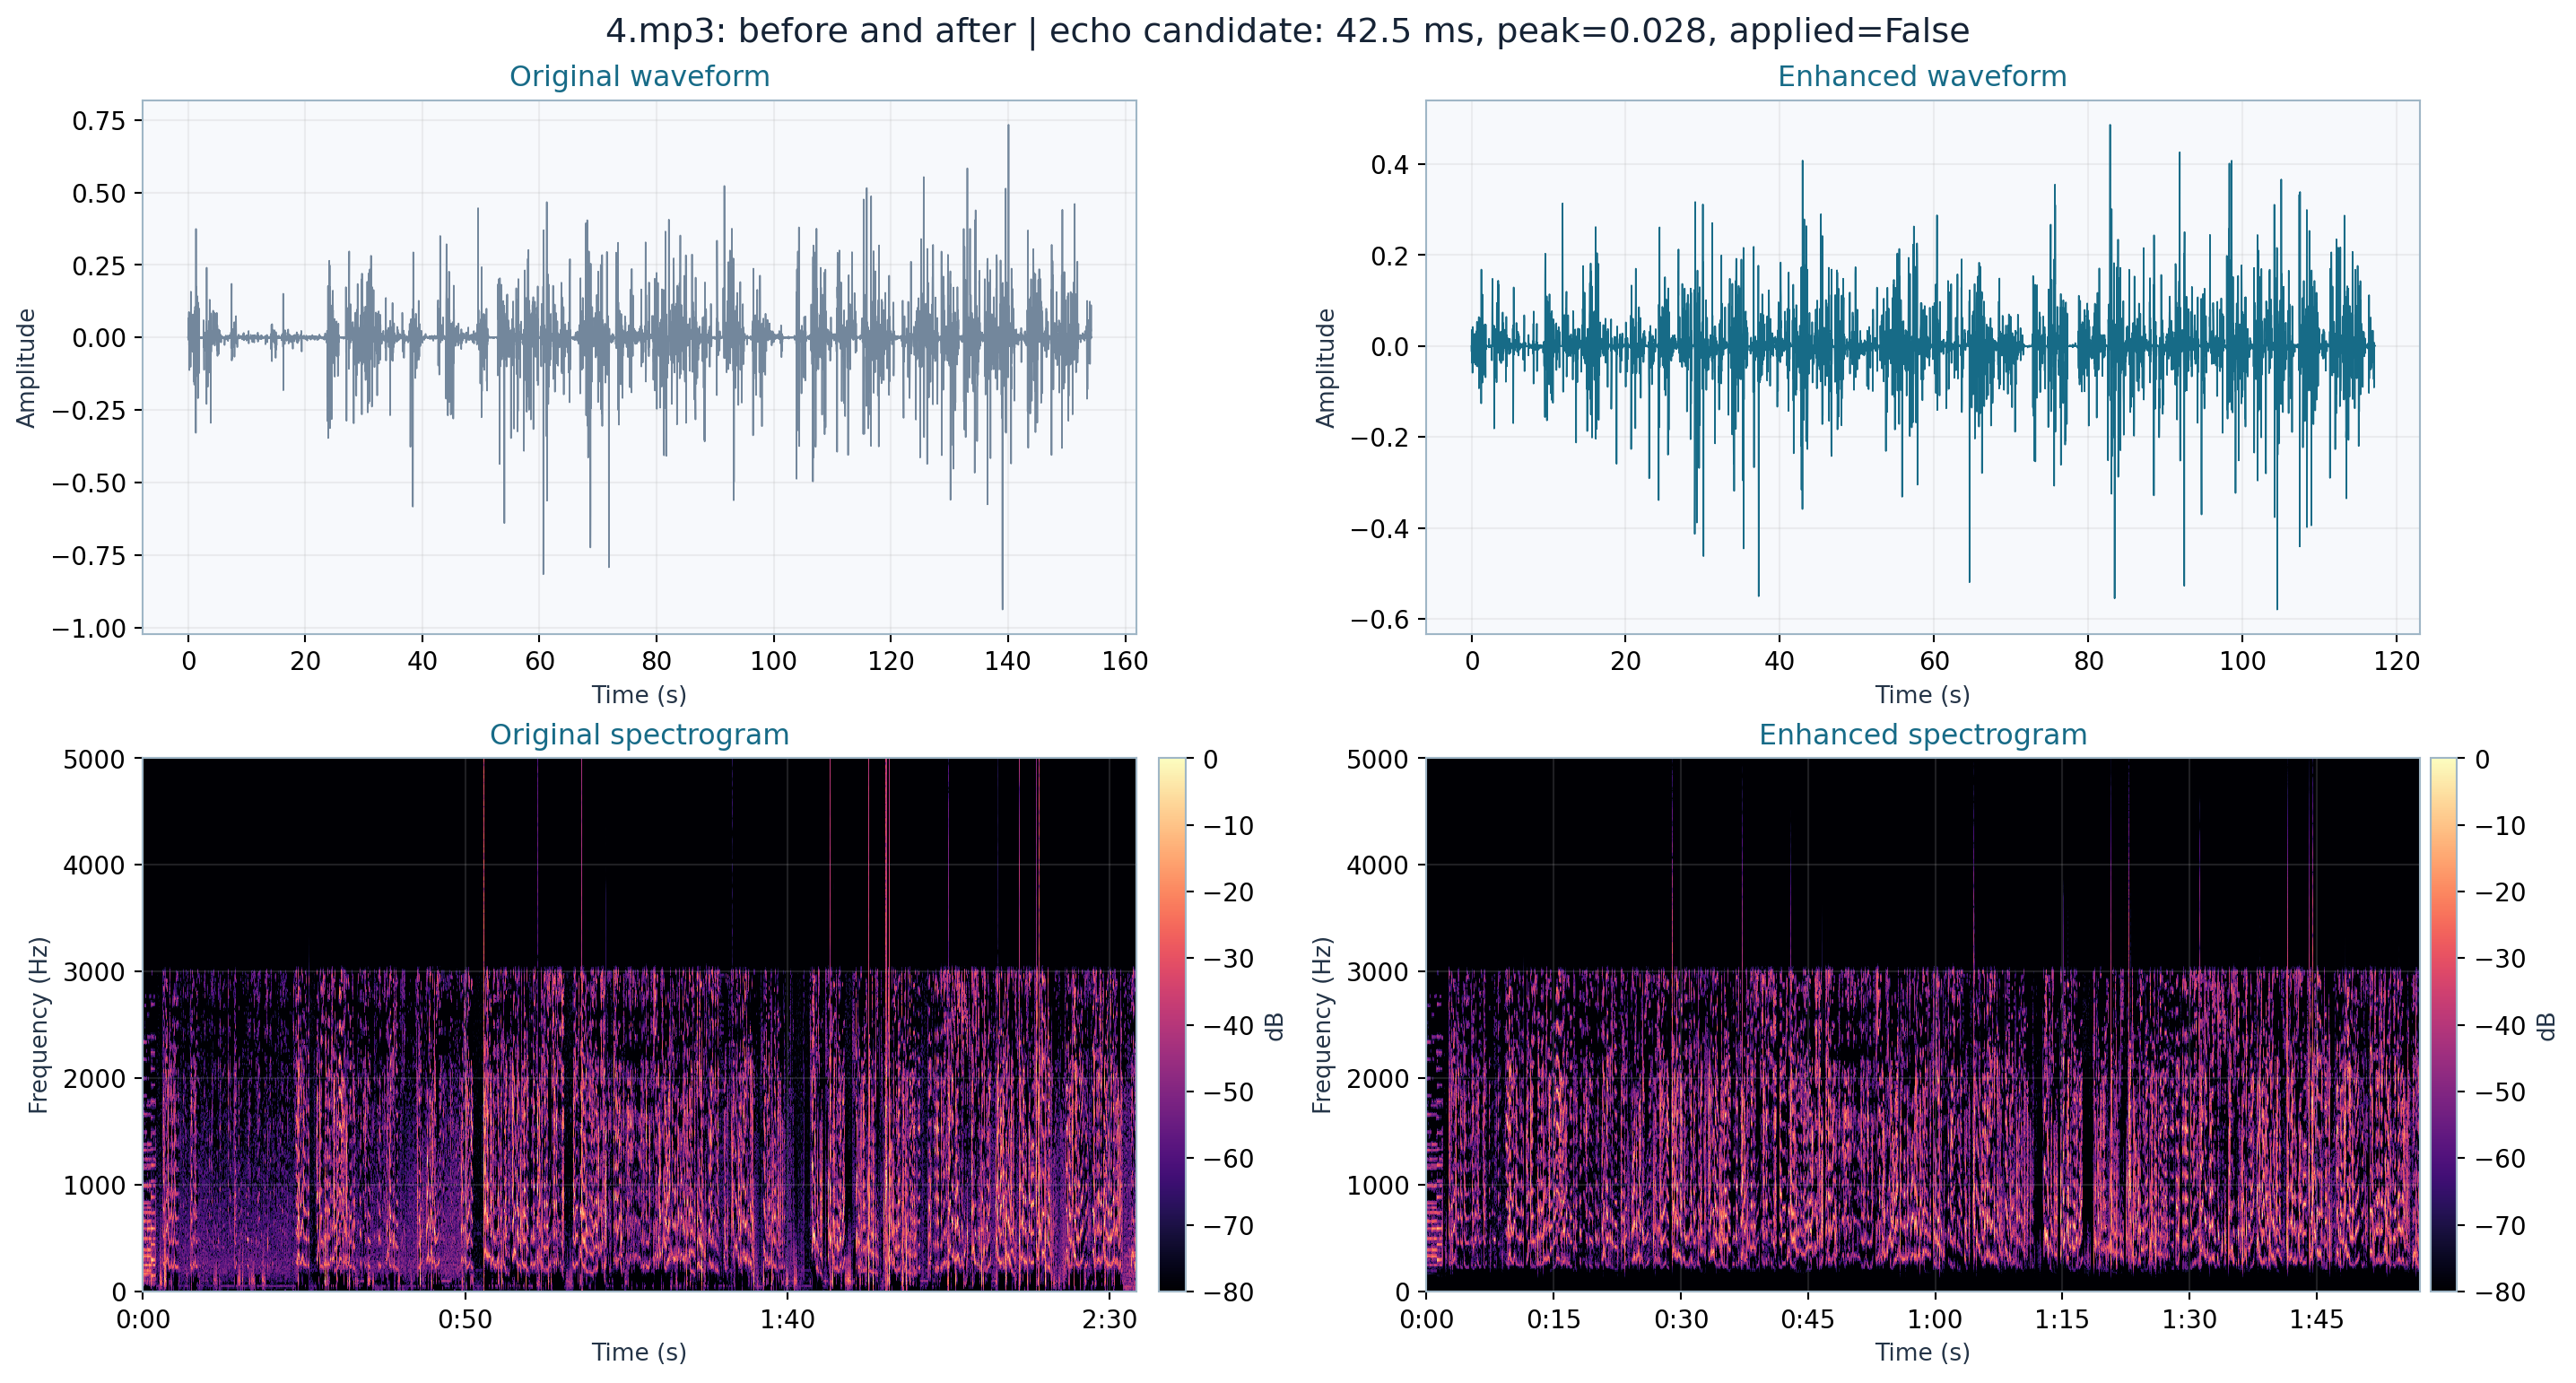
\includegraphics[width=0.96\textwidth]{audio_4_before_after.png}
\caption{مقایسه‌ی موج زمانی و طیف‌نگاره‌ی فایل ۴}
\end{figure}

در این فایل هم سکوت‌های بلند حذف شدند و طول حدود ۲۴ درصد کم شد. چون سیگنال از اول داخل باند تلفنی بود، سهم انرژی باند از ۹۲.۳ به ۹۹.۶ درصد رسید. بهبود اصلیِ قابل شنیدن انتظار می‌رود از حذف سکوت و نویز زمینه باشد، نه از دست‌کاری شدید طیف.

\begin{ideaBox}[نکته‌ی مهم درباره‌ی معیارها]
هیچ صدای مرجعِ تمیزی در اختیار نداریم. بنابراین \en{SNR} گزارش‌شده یک معیار جایگزین است که نسبت انرژی فریم‌های فعال به فریم‌های آرام را می‌سنجد. این عدد برای مقایسه خوب است، ولی جای آزمون شنیداری را نمی‌گیرد.
\end{ideaBox}

\clearpage
\section{بخش دوم: جداسازی شکستگی‌های اصلی}

در تصویر بازشده‌ی دیواره‌ی چاه، شکستگی صفحه‌ای معمولاً به صورت یک منحنی بلند یا سینوسی دیده می‌شود. مشکل این است که تصویر پر از ترک ریز، بافت و نوار عمودی است. پس فقط تیره‌بودن پیکسل کافی نیست.

مراحل اصلی این بخش این‌ها بودند:

\begin{enumerate}[rightmargin=7mm,itemsep=4pt]
  \item تبدیل به خاکستری و تقویت کنتراست محلی با \en{CLAHE}.
  \item هموارسازی ناهمسان‌گرد؛ کمی بیشتر در راستای افقی تا نوارهای عمودی ضعیف شوند.
  \item ساخت پاسخ رگه با \en{black-hat} برای خطوط تیره و \en{top-hat} برای خطوط روشن.
  \item ترکیب پاسخ رگه با گرادیان \en{Sobel} عمودی تا ساختارهای عمدتاً افقی امتیاز بیشتری بگیرند.
  \item بازکردن مورفولوژیک برای حذف نقاط و ترک‌های خیلی نازک، حذف مؤلفه‌های عمودی و سپس بستن افقی برای وصل‌کردن شکاف‌های کوتاه.
  \item تحلیل اجزای هم‌بند با معیارهای مساحت، کشیدگی، پوشش ستون‌ها و پهنای افقی.
\end{enumerate}

\begin{resultBox}[چرا دو قطب روشن و تیره بررسی شد؟]
دو تصویر اصلی شکستگی‌های تیره دارند، اما چند تصویر اضافی شکستگی روشن دارند. الگوریتم هر دو حالت را امتیاز می‌دهد و حالتی را انتخاب می‌کند که ساختارهای پیوسته‌تر و افقی‌تری ساخته است. برای هر دو تصویر اصلی، حالت تیره با فاصله‌ی مناسب برنده شد.
\end{resultBox}

\clearpage
\section{مراحل پردازش تصویر \en{Well1}}

\begin{figure}[ht]
\centering
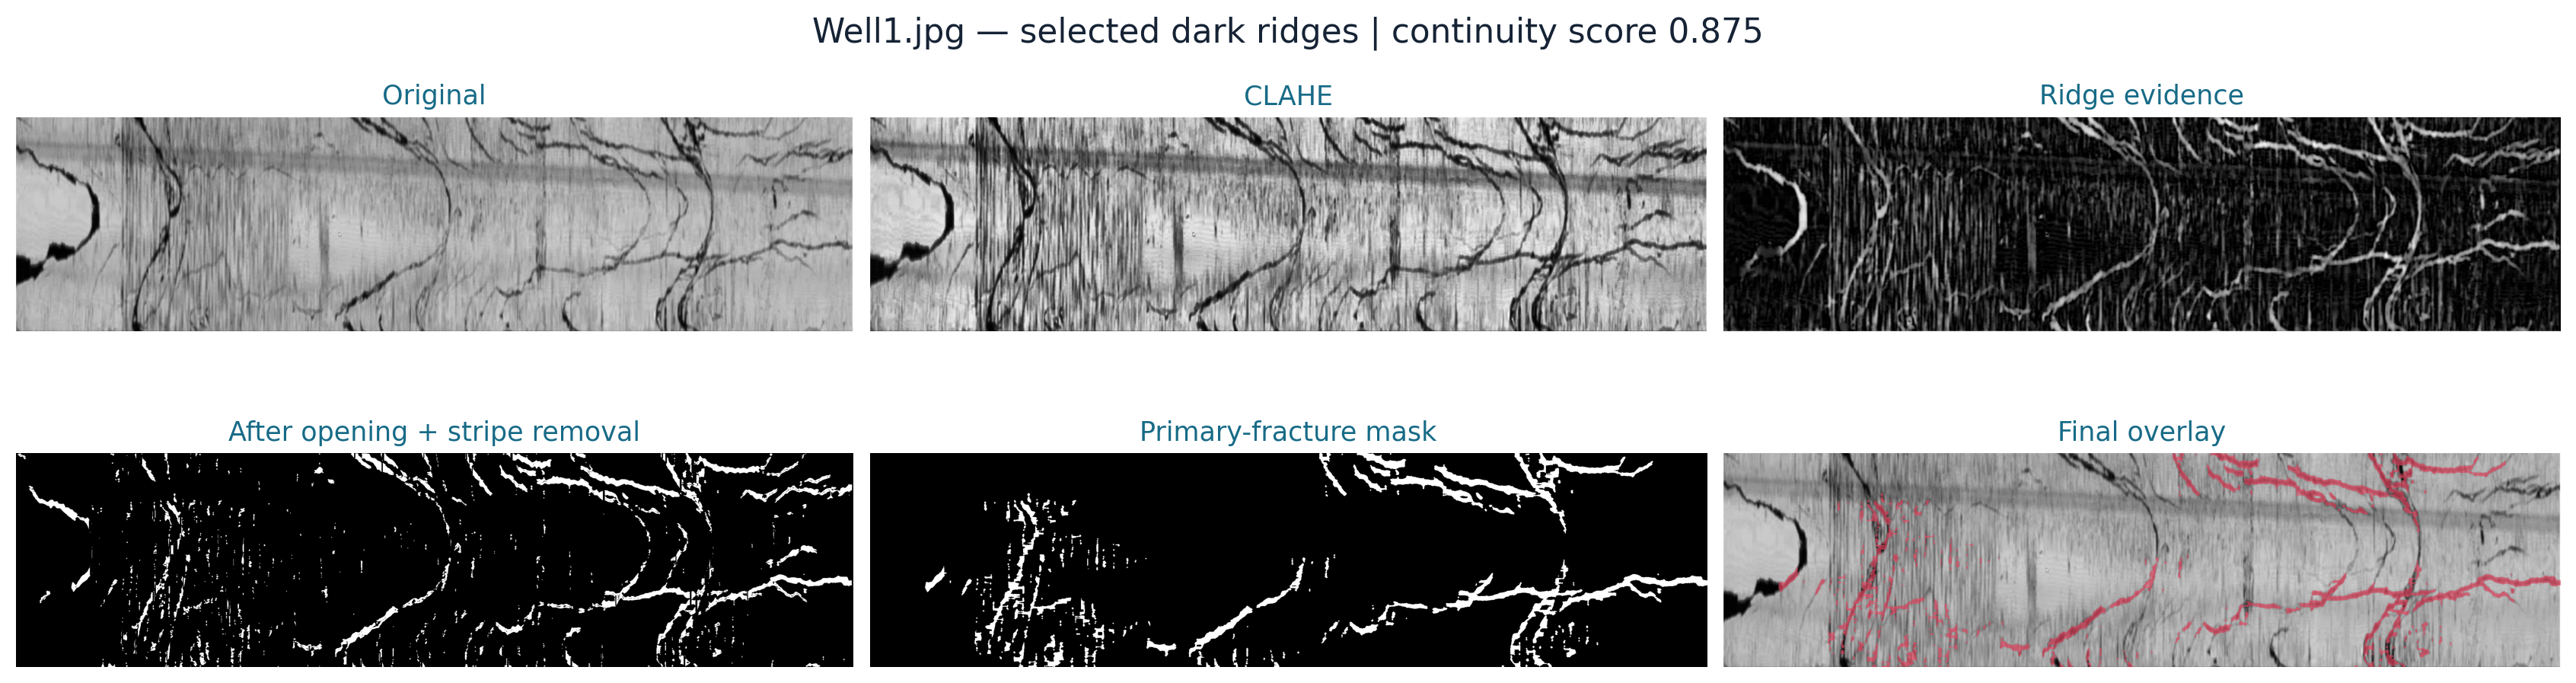
\includegraphics[width=\textwidth]{image_Well1_stages.png}
\caption{از تصویر خام تا ماسک و هم‌پوشانی نهایی برای \en{Well1.jpg}}
\end{figure}

در پاسخ رگه تقریباً همه‌ی ترک‌ها و بخشی از نوارهای عمودی دیده می‌شوند. بعد از بازکردن و حذف ساختار عمودی، بخش زیادی از بافت ریز کنار می‌رود. در ماسک نهایی فقط پیکسل‌های با اطمینان بالا داخل اجزایی نگه داشته شدند که آزمون پیوستگی را رد نکردند.

برای این تصویر چهار مؤلفه پذیرفته شد. بیشترین پهنای افقی برابر \metric{۴۶.۱ درصد} عرض تصویر بود و حدود \en{6.61\%} پیکسل‌ها در ماسک نهایی قرار گرفتند. این مقدار کم‌وبیش همان چیزی است که می‌خواهیم: شکستگی‌های اصلی دیده شوند، ولی کل بافت سنگ قرمز نشود.

\begin{ideaBox}[محدودیت دیده‌شده]
در بخش چپ تصویر هنوز تعدادی اثر عمودی کوتاه باقی مانده است. چون بعضی از آن‌ها به یک شکستگی پذیرفته‌شده وصل می‌شوند، تحلیل جزء هم‌بند آن‌ها را کاملاً جدا نمی‌کند. برای نسخه‌ی بعد می‌توان از تحلیل جهت محلی یا اسکلت‌بندی همراه با حذف شاخه‌های عمودی استفاده کرد.
\end{ideaBox}

\clearpage
\section{مراحل پردازش تصویر \en{well2}}

\begin{figure}[ht]
\centering
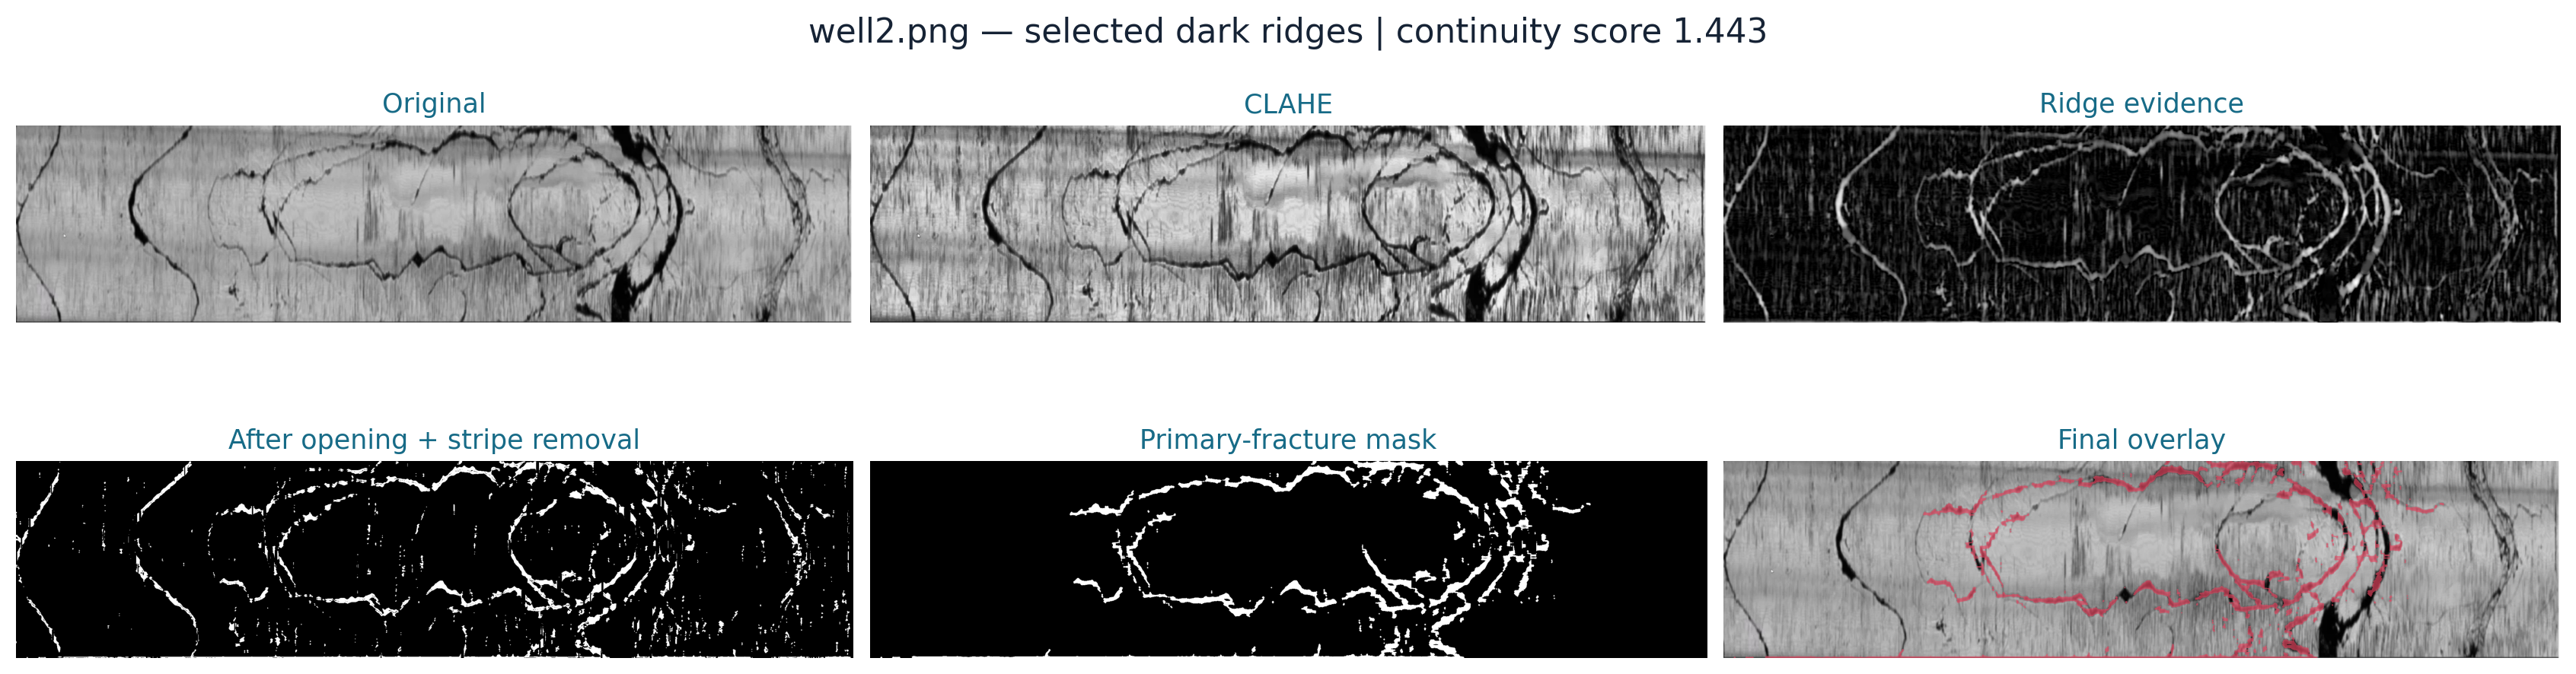
\includegraphics[width=\textwidth]{image_well2_stages.png}
\caption{از تصویر خام تا ماسک و هم‌پوشانی نهایی برای \en{well2.png}}
\end{figure}

رد سینوسی در این تصویر خیلی واضح‌تر است. الگوریتم دو مؤلفه را پذیرفت و بزرگ‌ترین مؤلفه حدود \metric{۸۴.۸ درصد} عرض تصویر را پوشش داد. فقط \en{6.13\%} پیکسل‌ها انتخاب شدند، اما مسیر بلند شکستگی تقریباً در سراسر تصویر دنبال شده است.

\begin{table}[ht]
\centering
\caption{خلاصه‌ی نتیجه‌ی دو تصویر اصلی}
\rowcolors{2}{softgray}{white}
\begin{tabular}{c c c c c}
\toprule
تصویر & قطب انتخابی & تعداد جزء & بیشترین پوشش افقی & پیکسل انتخابی\\
\midrule
\en{Well1.jpg} & تیره & ۴ & \en{46.1\%} & \en{6.61\%}\\
\en{well2.png} & تیره & ۲ & \en{84.8\%} & \en{6.13\%}\\
\bottomrule
\end{tabular}
\end{table}

\clearpage
\section{مقایسه‌ی نهایی دو تصویر اصلی}

\begin{figure}[ht]
\centering
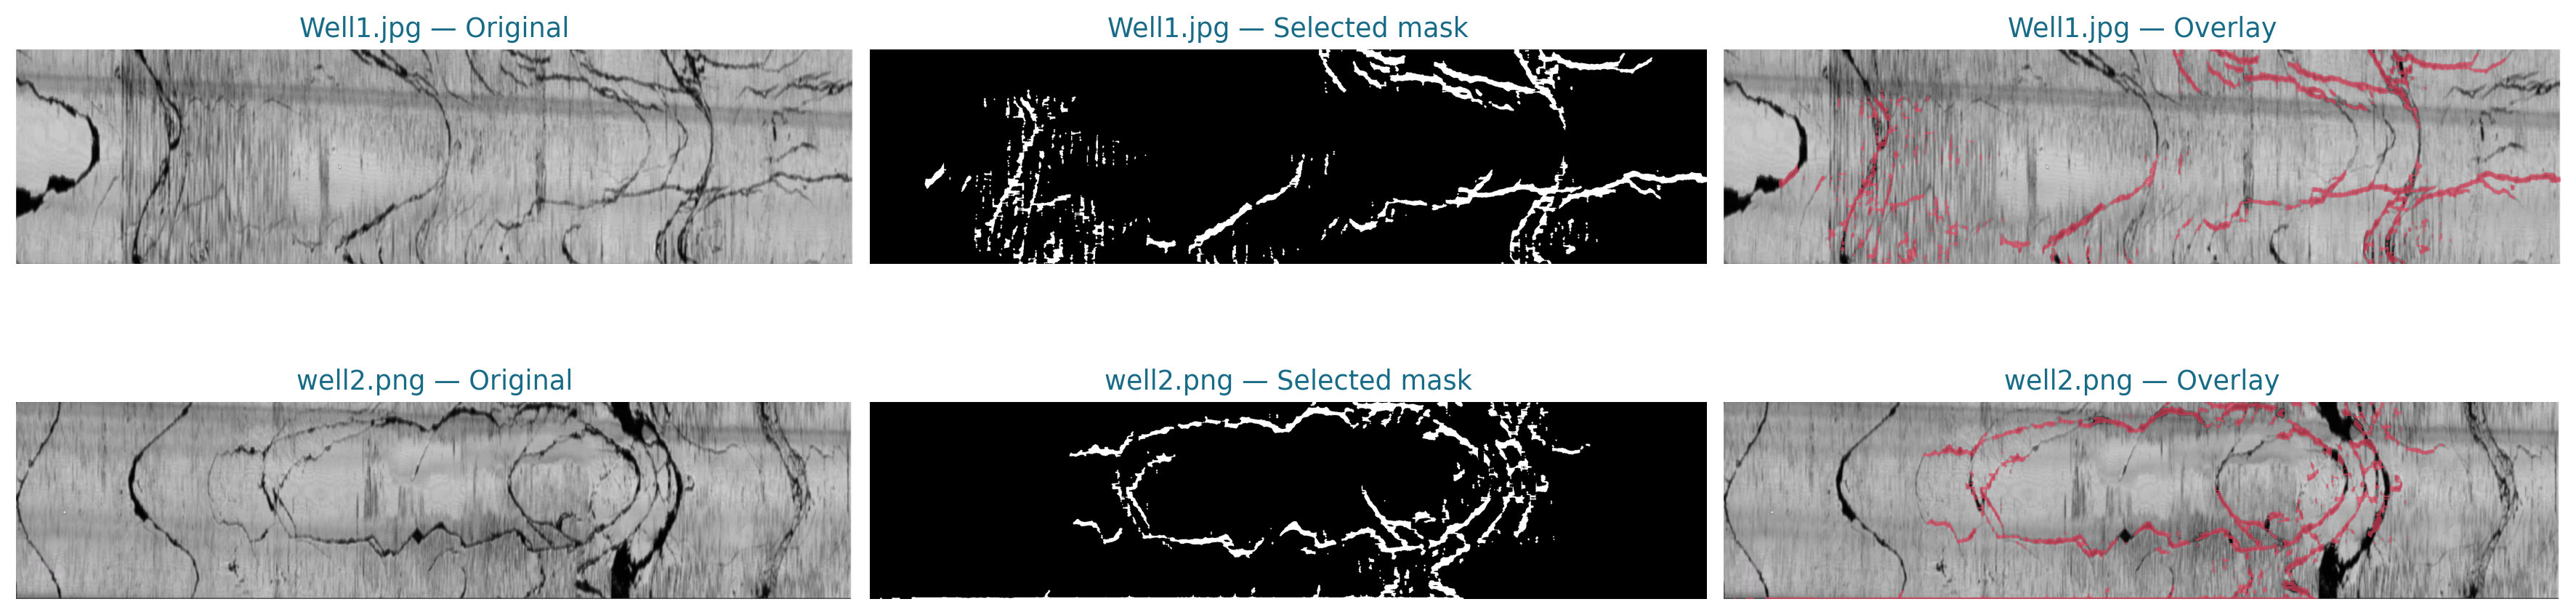
\includegraphics[width=\textwidth]{image_primary_comparison.png}
\caption{تصویر خام، ماسک انتخابی و هم‌پوشانی نهایی برای هر دو چاه}
\end{figure}

نکته‌ی مثبت این است که ماسک به جعبه‌ی محدودکننده‌ی اجزای پذیرفته‌شده تبدیل نشده است. بستن مورفولوژیک فقط برای آزمون پیوستگی استفاده شد و در خروجی نهایی دوباره به پیکسل‌های رگه‌ی با اطمینان بالا برگشتیم. در نتیجه نوارهای پهن و مصنوعی روی تصویر ساخته نشدند.

اگر داده‌ی برچسب‌خورده داشتیم، معیارهایی مثل دقت، یادآوری و \en{IoU} بهترین راه ارزیابی بودند. اینجا چون ماسک مرجع نداریم، پهنای افقی، پوشش ستون‌ها و نسبت پیکسل انتخابی نقش کنترل کیفیت را دارند.

\clearpage
\section{آزمون روی تصاویر اضافه}

\begin{figure}[ht]
\centering
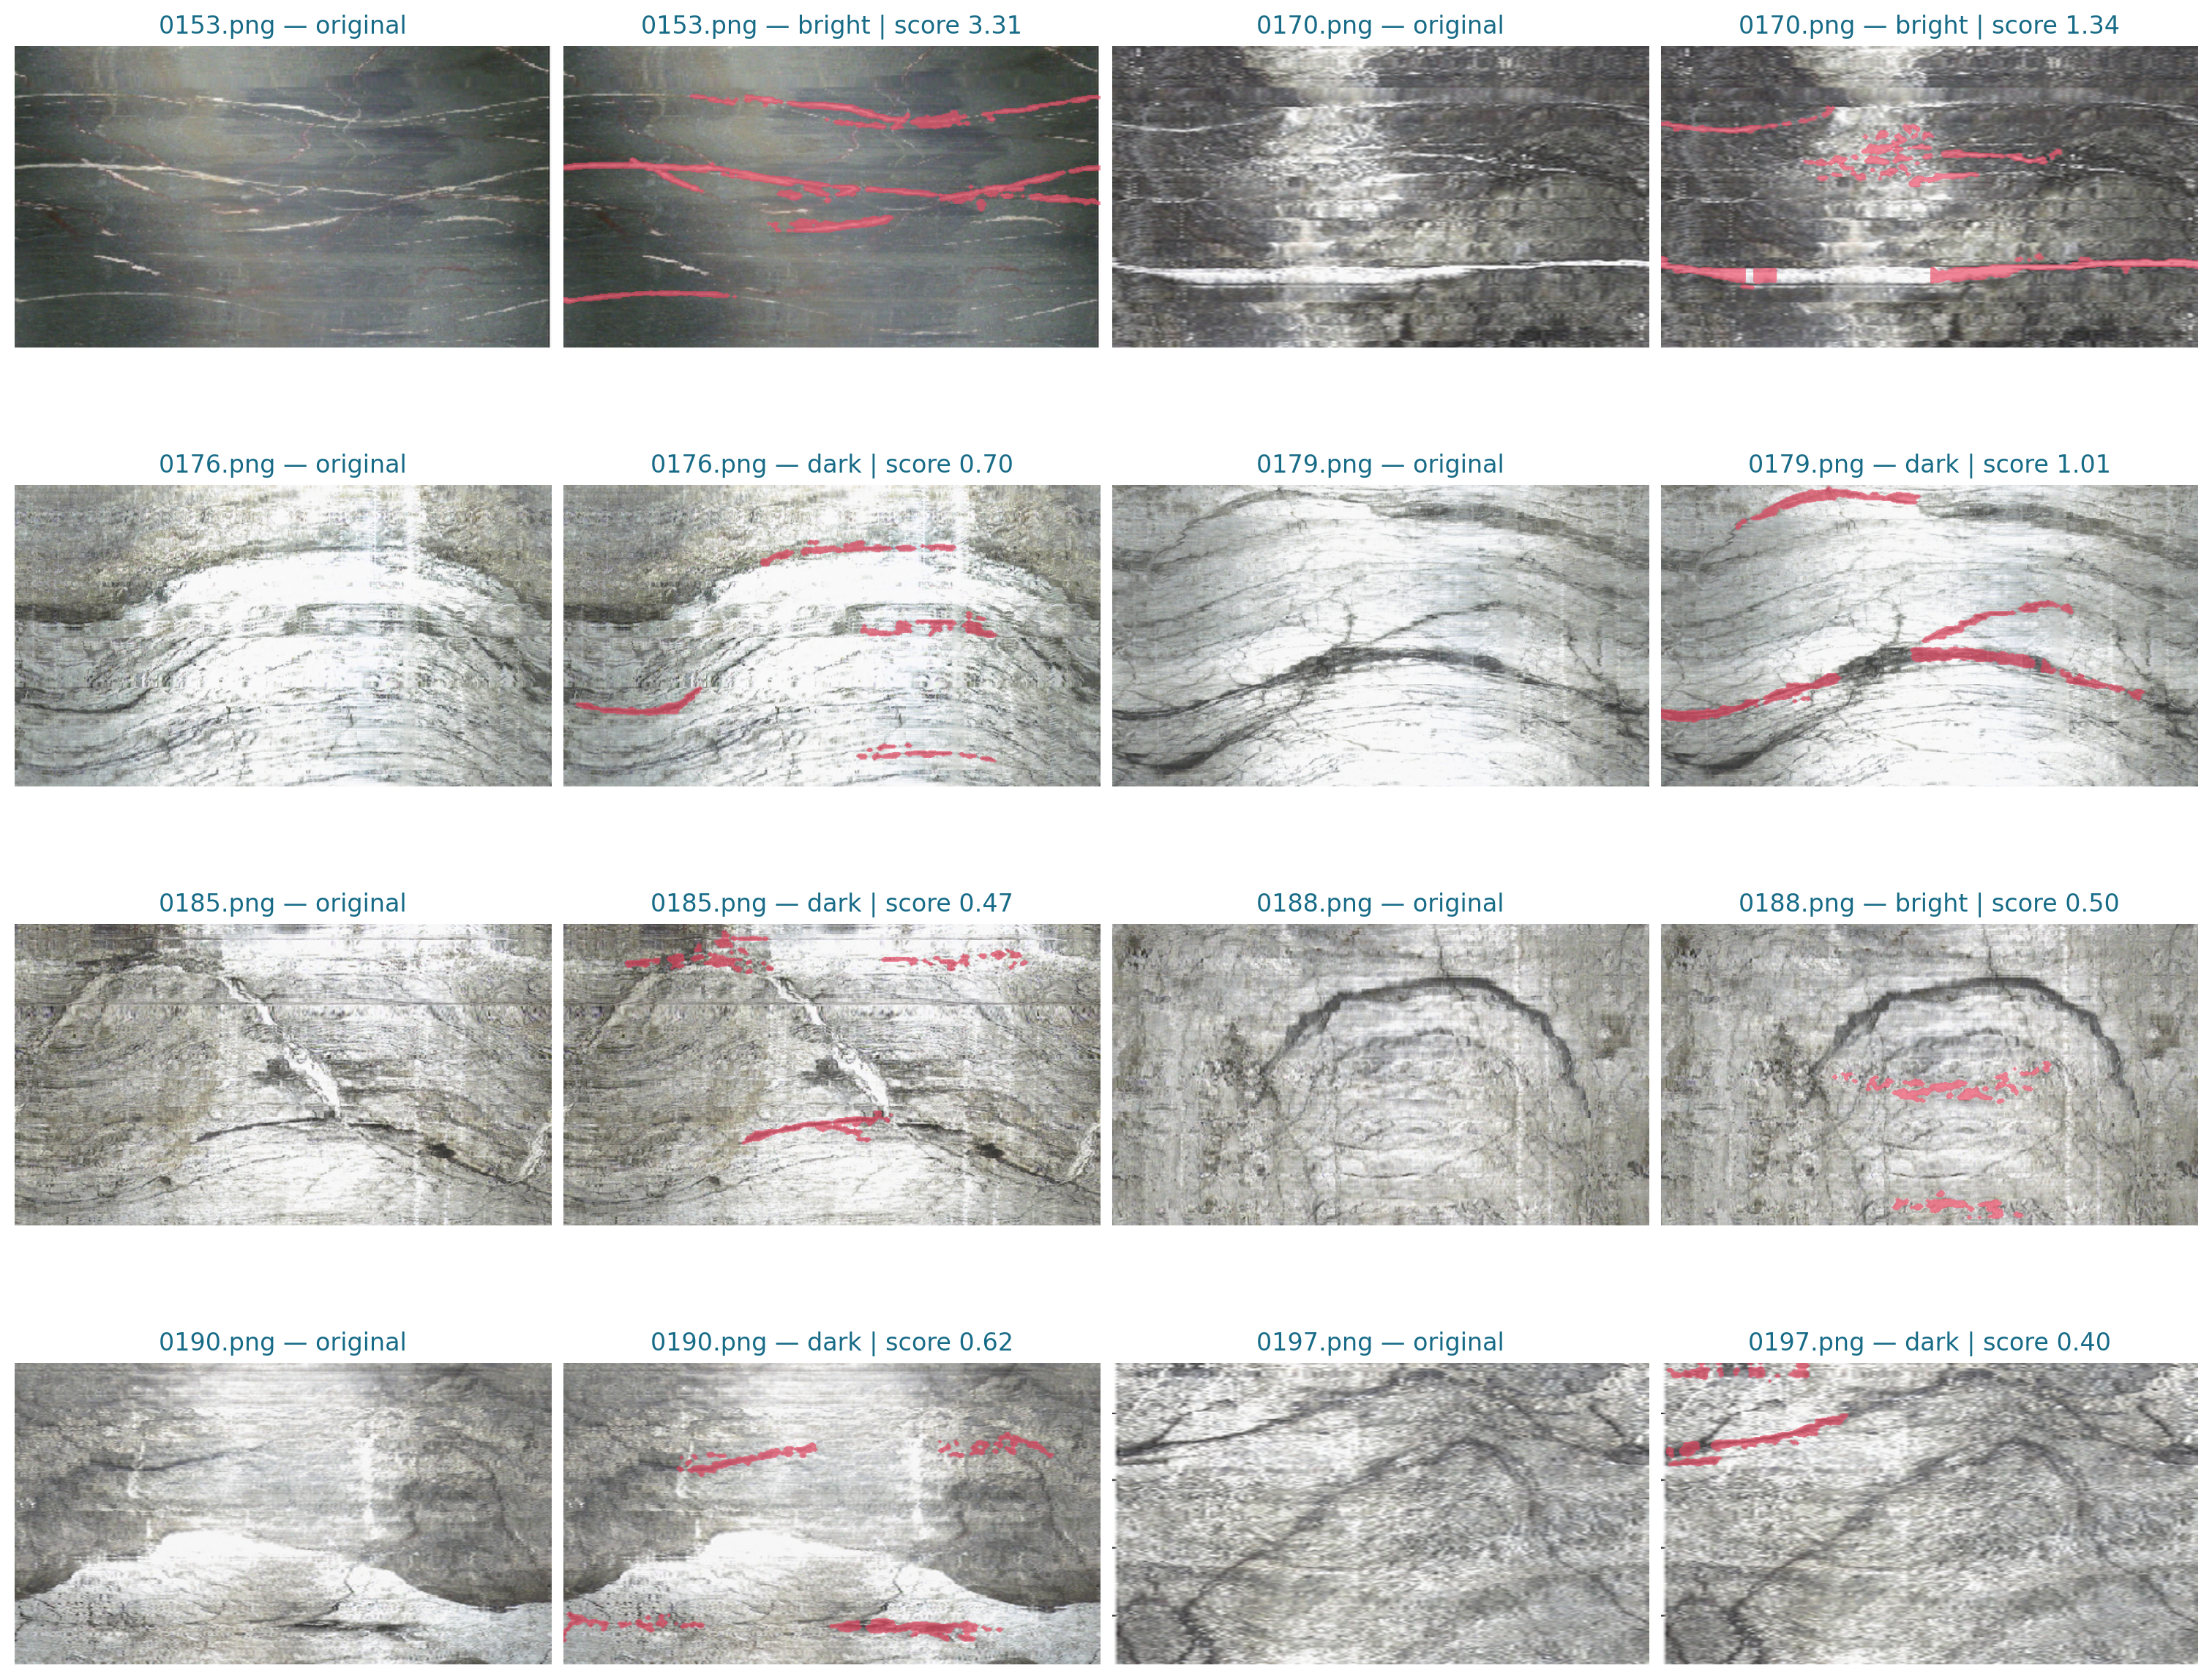
\includegraphics[width=\textwidth]{image_validation_montage.png}
\caption{اجرای همان تنظیمات روی هشت تصویر اضافه؛ سمت چپ هر جفت تصویر خام و سمت راست هم‌پوشانی خروجی است.}
\end{figure}

در تصویرهای \en{0153} و \en{0170} الگوریتم حالت روشن را انتخاب کرد و در بیشتر نمونه‌های دیگر حالت تیره برنده شد. این انتخاب خودکار نشان می‌دهد روش فقط به دو تصویر اصلی قفل نشده است.

با این حال نتیجه‌ها بی‌نقص نیستند. برای نمونه، نوار روشن و افقی می‌تواند از نظر پیوستگی شبیه شکستگی باشد. این دقیقاً جایی است که داشتن چند ماسک دستی یا یک فیلتر رگه‌ی هسیَن می‌تواند مرحله‌ی بعدی کار باشد.

\clearpage
\section{جمع‌بندی ارائه‌ای}

\begin{resultBox}[چیزهایی که خوب جواب دادند]
\begin{itemize}[rightmargin=5mm,itemsep=3pt]
  \item حذف سکوت بلند در فایل‌های ۲ و ۴ بدون بریدن کلمه‌ها.
  \item تمرکز انرژی صوت روی باند استاندارد گفتار و کنترل پیک خروجی.
  \item افزایش واضح \en{SNR} تخمینی در فایل‌های ۲ و ۴.
  \item پیدا کردن ردهای بلند و سینوسی در دو تصویر اصلی.
  \item استفاده از یک کد مقیاس‌پذیر روی تصاویر اصلی و نمونه‌های کوچک‌تر.
\end{itemize}
\end{resultBox}

\begin{ideaBox}[سخت‌ترین بخش‌ها]
اکو و موسیقی انتظار بیشترین هم‌پوشانی را با گفتار دارند، پس حذف کامل آن‌ها با یک فیلتر ساده واقع‌بینانه نیست. در تصویر هم بافت‌های قوی و نوار روشن می‌توانند از نظر هندسی شبیه شکستگی باشند. در هر دو مسئله، راه‌حل محافظه‌کارانه انتخاب شد تا محتوای اصلی کمتر آسیب ببیند.
\end{ideaBox}

اگر بخواهیم پروژه را یک مرحله جلوتر ببریم، برای صوت می‌توان از فیلتر وینر تطبیقی یا برآورد اکو روی بازه‌های گفتار جداگانه استفاده کرد. برای تصویر هم بهترین ادامه، ساخت چند ماسک مرجع و تنظیم آستانه‌ها با معیارهای واقعی است.

% \vfill
% \begin{center}
% \begin{tcolorbox}[
%   width=0.88\textwidth,
%   colback=deepblue,
%   colframe=deepblue,
%   arc=3mm,
%   boxrule=0pt
% ]
% \centering\color{white}\large\bfseries
% نتیجه‌ی اصلی: اول اندازه‌گیری کردیم، بعد تصمیم گرفتیم، و هر تصمیم را با شکل یا عدد قابل بررسی نگه داشتیم.
% \end{tcolorbox}
% \end{center}

\end{document}
